\section{Results}
\begin{figure}[ht]\centering
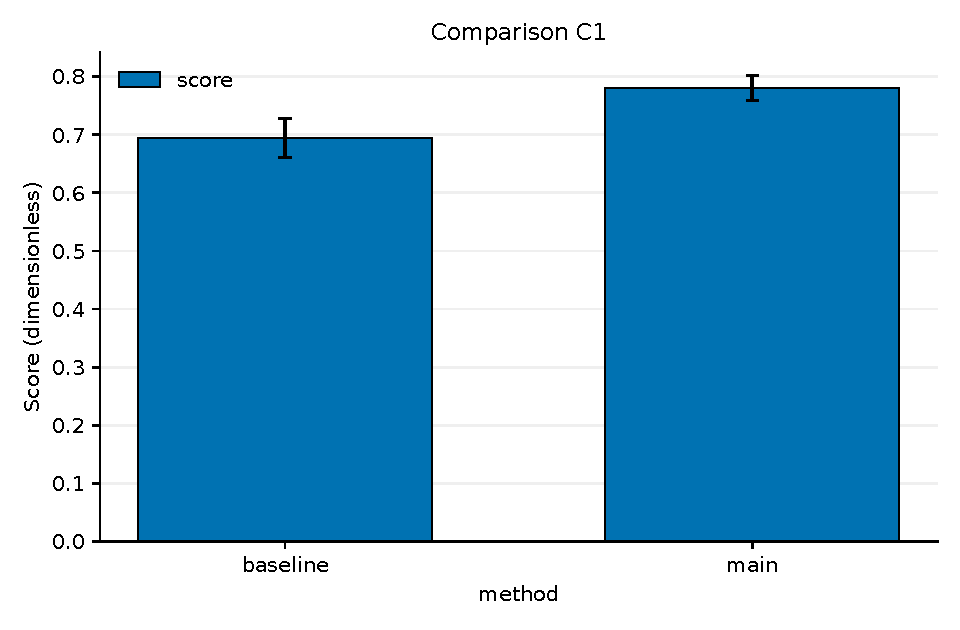
\includegraphics[width=4in]{figures/fig_c1.pdf}
\caption{Recorded comparison; error bars show confidence intervals.}\label{fig:fig_c1}\end{figure}
\begin{figure}[ht]\centering
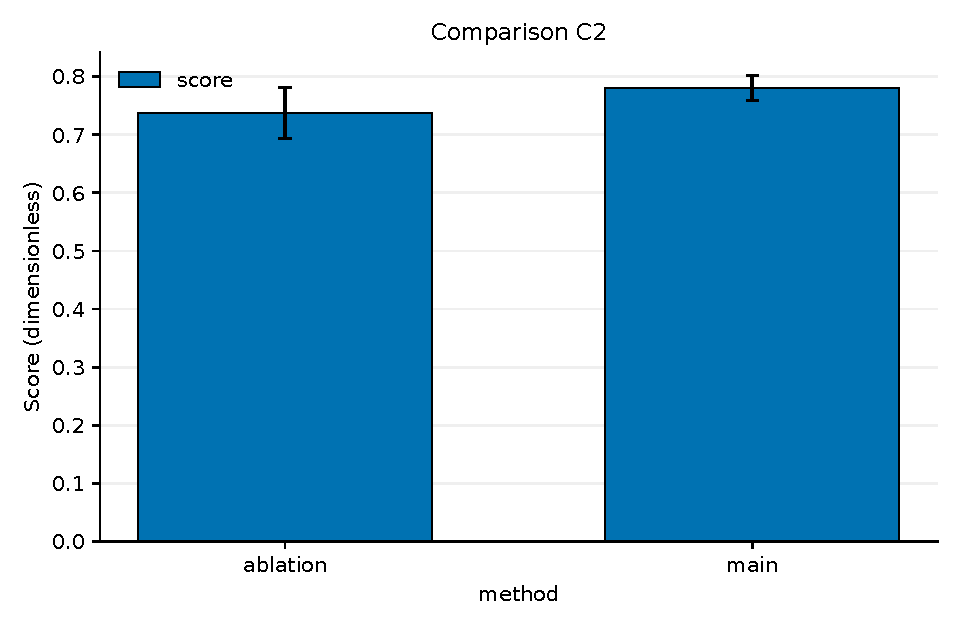
\includegraphics[width=4in]{figures/fig_c2.pdf}
\caption{Recorded comparison; error bars show confidence intervals.}\label{fig:fig_c2}\end{figure}

\claim{CL1}{Comparison C1: the observed mean difference is \airval{C1.score.diff_mean.9eadf13e2a039f1b7e2313fd9ad4dfb3f21e3bc86934d785e6ba925c788cd4aa}, with p-value \airval{C1.score.p_value.54cab263c0d6d3f64fbe3d6a239aad878d9e7193cb49473637db99469dfce5b0} and \airval{C1.score.n.517677a0852f928687d4c0b93c3c8745b67ce5c6e0c52d3be762326f19e8b789} seeds in the first group. This observation is limited to the evaluated scope.}
\claim{CL2}{Comparison C2: the observed mean difference is \airval{C2.score.diff_mean.4a76d41d55937b1d2f48da34d7d2acbed5eb13471d8ae1a0f7636bbc5ef83df5}, with p-value \airval{C2.score.p_value.7adea3319eea07c8199a41d454bbf001b1c7cb0fd3e825cb83c59fae7676f8a9} and \airval{C2.score.n.85d42dd3a8caae90f7e422eadb9a47ce46cff5e140dbaed7100278f9bf8697e9} seeds in the first group.}
